%\documentclass{article}
%\documentclass[hyperref={colorlinks=true}]{beamer}
%\documentclass[handout,hyperref={colorlinks=true}]{beamer}
\documentclass[handout,hyperref={colorlinks=true}]{beamer}
\usecolortheme{crane}
\usetheme{Madrid}
\usefonttheme{structuresmallcapsserif}

%%%%%%%%%%%%%%%%%%%%%%%%%%%%%%Paquetes%%%%%%%%%%%%%%%%%%%%%%%%%%%%%%%%%%%%%%%%%%%%%%%5
%%%%%%%%%%%%%%%%%%%%%%%%%%%%%%%%%%%%%%%%%%%%%%%%%%%%%%%%%%%%%%%%%%%%%%%%%%%%%%%%%%%%%

%\usepackage{pgfpages}
%\pgfpagesuselayout{4 on 1}[a4paper,landscape,border shrink=5mm]
\usepackage{empheq}
\usepackage[spanish]{babel}
\usepackage[utf8x]{inputenc}
\usepackage{times}
\usepackage[T1]{fontenc}
\usepackage{amssymb,amsmath}
\usepackage{enumerate}
\usepackage{verbatim}
\usepackage{ esint }
\usepackage{pdfsync}
%\usepackage{pst-all}
%\usepackage{pstricks-add}
\usepackage{array}
%\usepackage[T1]{fontenc}
\usepackage{animate}
%\usepackage{media9}
%\usepackage{movie15}
\usepackage{xparse}
\usepackage{listings}
\usepackage{ wasysym }
\usepackage{sagetex}
\usepackage{hyperref}




%%%%%%%%%%%%%%%%%%%%%%%%%Configuracion listing
\lstdefinelanguage{Sage}[]{Python}
{morekeywords={False,sage,True},sensitive=true}
\lstset{
  frame=none,
  showtabs=False,
  showspaces=False,
  showstringspaces=False,
  commentstyle={\ttfamily\color{dgreencolor}},
  keywordstyle={\ttfamily\color{dbluecolor}\bfseries},
  stringstyle={\ttfamily\color{dgraycolor}\bfseries},
  language=Sage,
  basicstyle={\fontsize{8pt}{8pt}\ttfamily},
  aboveskip=.3em,
  belowskip=0.1em,
  numbers=none,
  numberstyle=\footnotesize
}


 


%%%%%%%%%%%%%%%%%%%%%%%%Colores
\definecolor{myblue}{rgb}{.8, .8, 1}
\definecolor{dblackcolor}{rgb}{0.0,0.0,0.0}
\definecolor{dbluecolor}{rgb}{0.01,0.02,0.7}
\definecolor{dgreencolor}{rgb}{0.2,0.4,0.0}
\definecolor{dgraycolor}{rgb}{0.30,0.3,0.30}
\newcommand{\dblue}{\color{dbluecolor}\bf}
\newcommand{\dred}{\color{dredcolor}\bf}
\newcommand{\dblack}{\color{dblackcolor}\bf}



\newtheorem{thm}{Teorema}






%%%%%%%%%%%%%%%%%%%%%%%%%%Nuevos comandos entornos%%%%%%%%%%%%%%%%%%%%%%%%%%%%%%%%
%%%%%%%%%%%%%%%%%%%%%%%%%%%%%%%%%%%%%%%%%%%%%%%%%%%%%%%%%%%%%%%%%%%%%%%%
\newenvironment{demo}{\noindent\emph{Dem.}}{$\square$ \newline\vspace{5pt}}
\newcommand{\com}{\mathbb{C}}
\newcommand{\dis}{\mathbb{D}}
\newcommand{\rr}{\mathbb{R}}
\newcommand{\oo}{\mathcal{O}}
\renewcommand{\emph}[1]{\textcolor[rgb]{1,0,0}{#1}}
\newcommand{\der}[2]{\frac{\partial #1}{\partial #2}}
\renewcommand{\v}[1]{\overrightarrow{#1}}
\renewcommand{\epsilon}{\varepsilon}
\newlength\mytemplen
\newsavebox\mytempbox
\makeatletter
\newcommand\mybluebox{%
    \@ifnextchar[%]
       {\@mybluebox}%
       {\@mybluebox[0pt]}}

\def\@mybluebox[#1]{%
    \@ifnextchar[%]
       {\@@mybluebox[#1]}%
       {\@@mybluebox[#1][0pt]}}

\def\@@mybluebox[#1][#2]#3{
    \sbox\mytempbox{#3}%
    \mytemplen\ht\mytempbox
    \advance\mytemplen #1\relax
    \ht\mytempbox\mytemplen
    \mytemplen\dp\mytempbox
    \advance\mytemplen #2\relax
    \dp\mytempbox\mytemplen
    \colorbox{myblue}{\hspace{1em}\usebox{\mytempbox}\hspace{1em}}}

\makeatother
\DeclareDocumentCommand\boxedeq{ m g }{%
    {\begin{empheq}[box={\mybluebox[2pt][2pt]}]{equation}% #1%
        \IfNoValueF {#2} {\label{#2}}%
       #1
       \end{empheq}
    }%
}
\DeclareMathOperator{\mcd}{mcd}
\DeclareMathOperator{\atan2}{atan2}
\DeclareMathOperator{\sen}{sen}
\newtheorem{teorema}{Teorema}[section]
\newtheorem{lema}[teorema]{Lema}
\newtheorem{corolario}[teorema]{Corolario}
\newtheorem{proposicion}[teorema]{Proposici\'on}
\newtheorem{definicion}[teorema]{Definici\'on}
%%%%%%%%%%%%%%%%%%%%%%%%%%%%%%%%%%%%%%%%%%%%%%%%%%%%%%%%%%%%%%%%%%%%%%%%%%%%%%%%%%%%%%%%%%%%%%%%%%%%%%%%%%%




%%%%%%%%%%Para escibir en clase articulo o similar
% \usepackage{color}
% \newcommand{\nl}{ }
% \renewenvironment{frame}[1]{}{}
% \newcommand{\qed}{$\square$}
% %\newcommand{\defverbatim}{\def{#1}}
% \newenvironment{block}[1]{\textbf{#1}}{}
% \title{Ecuaciones lineales de segundo orden}
% \author{Fernando Mazzone}
% 




%%%%%%%%%%%%%%%%%%%%%%%Para clase beamer
\newcommand{\nl}{\onslide<+-> }
% \mode<all>
% {
%   \usetheme{Boadilla}
%   % oder ...
%  
%   \setbeamercovered{wolverine}
%   % oder auch nicht
% }


%\mode<handout>{
%  \usetheme{default}
  %\setbeamercolor{background canvas}{bg=black!5}
 % \pgfpagesuselayout{2 on 1}[a4paper,landscape,border shrink=2.5mm]
%}

% \mode<all>{
%   \usetheme{default}
%   %\setbeamercolor{background canvas}{bg=black!5}
%   \pgfpagesuselayout{4 on 1}[letterpaper,landscape,border shrink=2.5mm]
% }

\title[Ecuaciones lineales de segundo orden] % (optional, nur bei langen Titeln nötig)
{%
 Ecuaciones lineales de segundo orden
}



\author[] % (optional, nur bei vielen Autoren)
{Fernando Mazzone}

\institute% (optional, aber oft nötig)
{
 Depto de Matemática\\
Facultad de Ciencias Exactas Físico-Químicas y Naturales\\
Universidad Nacional de Río Cuarto}


\subject{Ecuaciones Diferenciales}

%%%%%%%%%%%%%%%%%%%%%%%%%%%%%%%%%%%%%%%%%%%%%%%%%%%%%%%%%%%%%%%%%%%%%%%%%%%%%%%%%%%%%%




\begin{document}

\section{Ecuaciones lineales de orden superior}

\begin{frame}{Ecuación lineal general de orden $n$}
\begin{block}{Ecuación lineal general de orden $n$}
Es una ecuación de la forma
\boxedeq{y^{(n)}(x)+p_{n-1}(x)y^{(n-1)}(x)+\cdots+p_0(x)y(x)=r(x)}{eq:ecua_lin_gen_orden_n}
donde $p_i,r$, $i=0,\ldots,n-1$ son funciones definidas en un intervalo $I$
\end{block}


Los resultados y técnicas que hemos desarollado para ecuaciones de orden $2$ se aplican con cambios menores a ecuaciones de mayor orden. No vamos a repetir la demostración de estos resultados, dado que es prácticamente la misma que para el caso $n=2$. Los exponemos de manera sumaria.
\end{frame}

\begin{frame}{Existencia y unicidad de soluciones}
\begin{block}{Teorema de existencia y unicidad de soluciones}
 Supongamos $p_i,r$, $i=0,\ldots,n-1$ continuas sobre $I$. Sean $x_0\in I$ e $y_0,y_1,\ldots y_{n-1}\in\rr$ dados. Entonces existe una única solución del PVI
 \[\left\{
 \begin{array}{l l l}
   y^{(n)}(x)+&p_{n-1}(x)y^{(n-1)}(x)+\cdots+p_0(x)y(x)=r(x),x\in I\\
   y(x_0)&=y_0&\\
   y'(x_0)&=y_1&\\
   &\vdots\\
  y^{(n-1)}(x_0)&=y_{n-1}&\\
  \end{array}\right.
\]

\end{block}
\end{frame}

\begin{frame}{Estructura del conjunto de soluciones}

\begin{block}{Teorema: estructura conjunto de soluciones ecuaciones homogéneas}
Supongamos $y_1,y_2,\ldots,y_n$ soluciones linealmente independientes de 
\[y^{(n)}(x)+p_{n-1}(x)y^{(n-1)}(x)+\cdots+p_0(x)y(x)=0.\]
Entonces 
\[y=c_1y_1+\cdots+c_ny_n,\quad c_i\in\rr, i=1,\ldots,n,\]
es solución general. Vale decir, el conjunto de soluciones es un espacio vectorial $n$-dimensional.
\end{block}
\end{frame}


\begin{frame}{Estructura del conjunto de soluciones}
\begin{block}{Teorema: estructura conjunto de soluciones ecuaciones no homogéneas}
Una solución general de la ecuación no homogénea  
\[y^{(n)}(x)+p_{n-1}(x)y^{(n-1)}(x)+\cdots+p_0(x)y(x)=r(x),\]
es la suma de una solución particular de esta ecuación más una solución general de la ecuación homogénea asociada.
\end{block}

\end{frame}




\begin{frame}{Wronskiano}
\begin{block}{Fórmula Abel}
Si $y_1,y_2,\ldots,y_n$ son soluciONES de la ecuación  homogénea  
\boxedeq{y^{(n)}(x)+p_{n-1}(x)y^{(n-1)}(x)+\cdots+p_0(x)y(x)=0,}{eq:lin_hom_orden_n}
Entonces el Wronskiano satisface
\boxedeq{W(y_1,\ldots,y_n)(x)=W(y_1,\ldots,y_n)(x_0)e^{-\int_{x_0}^xp_{n-1}(t)dt}.}{eq:formu_abel}
En particular  $\{y_1,y_2,\ldots,y_n\}$ son linalmente independientes si y solo si $W(x)\neq 0$ para todo $x\in I$.
\end{block}

\textbf{Dem.} Las demostraciones de los resultados anteriores es tan similar a su análogo de orden 2 que no vale la pena invertir tiempo en ellas. La demostración de la fórmula de Abel, si nos parece lo suficientemente interesante para dejarla como \textbf{Ejercicio}.
\end{frame}


\begin{frame}{Ecuaciones homogéneas con coeficientes constantes}
Las ecuaciones lineales de orden $n$, homogeneas con coeficientes constantes  se resuelven por métodos análogos a los considerados para ecuaciones de segundo orden. Se propone $y(x)=e^{rx}$ como solución. Reemplazando esta función
en \eqref{eq:lin_hom_orden_n} vemos que $y$ sería solución si y solo si $r$ es solución de la ecuación característica
\boxedeq{r^n+p_{n-1}r^{n-1}+\cdots+p_1r+p_0=0.}{eq:ecua_carac}
 
Ahora se presentan casos algo diferentes.


\end{frame}

\begin{frame}{Ecuaciones homogéneas con coeficientes constantes}\label{pag:oper1}

\textbf{Raices reales distintas.}
Si la ecuación característica \eqref{eq:ecua_carac} tiene $n$ raíces $r_1,\ldots,r_n$ reales y distintas entonces 
$y_1(x)=e^{r_1x},\ldots,y_n(x)=e^{r_nx}$ son soluciones linealmente independientes y por ende
\[\boxed{y(x)=c_1e^{r_1x}+\cdots+c_ne^{r_nx}}\]
es solución general. 

Dejamos como ejercicio la demostración de la independencia lineal. En lugar de usar el Wronskiano, se puede utilizar  la siguiente idea basada en métodos operacionales. 

Por $D$ vamos a denotar el operador diferenciación, esto es $D$ es sencillamente la función  definida sobre el conjunto de funciones diferenciables sobre un intervalo abierto y que actúa derivando, esto es $Dy=y'(x)$. 





\end{frame}





\begin{frame}{Ecuaciones homogéneas con coeficientes constantes}\label{pag:oper2}
Dado un polinomio $p(X)=p_nX^n+p_{n-1}X^{n-1}+\cdots+p_1X+p_0$, $p_i\in\rr$, $i=0,\ldots,n$, denotamos por  $p(D)$ el operador definido por
\[p(D)y=p_ny^{(n)}+p_{n-1}y^{(n-1)}+\cdots+p_1y'+p_0y.\]
Diremos que $p(D)$ es un \emph{operador diferencial polinomial}. 

\textbf{Ejercicio 1} Dado que dos polinomios se pueden sumar y multiplicar resultando estas operaciones en un nuevo polinomio, es posible hacer lo propio con operadores diferenciales polinomiales. Demostrar que el producto de dos de tales operadores  $p(D)$ y $q(D)$ es conmutativo. Esta propiedad es lo mismo que afirmar que el producto de polinomios es conmutativo. Analizar que ocurriría si permitiesemos que los coeficientes $p_i$ fuesen funciones de $x$, $p_i=p_i(x)$.
 
\end{frame}

\begin{frame}{Ecuaciones homogéneas con coeficientes constantes}\label{pag:oper3}

\textbf{Ejercicio 2} Supongamos ahora que $r_1,\ldots,r_n$ son números reales distintos y que 
\[y=c_1e^{r_1x}+c_2e^{r_2x}+\cdots+c_ne^{r_nx}.\]
Considerar el operador diferencial
\[p(D)=(D-r_1)\cdots(D-r_{i-1})(D-r_{i+1})\cdots(D-r_n).\]
Demostrar que
\[p(D)y=(r_i-r_1)\cdots(r_i-r_{i-1})(r_i-r_{i+1})\cdots(r_i-r_n)e^{r_ix}.\]
Deducir de esto la independencia lineal de $\{e^{r_1x},\ldots,e^{r_nx}\}$.
\end{frame}

\begin{frame}{Ecuaciones homogéneas con coeficientes constantes}
\textbf{Raices reales repetidas.}
Supongamos que la ecuación característica \eqref{eq:ecua_carac} tiene  raíces reales repetidas. Sean $r_1,\ldots,r_k$ las raices distintas y $m_j$ la multiplicidad de la raíz $r_j$. Por cada raíz $r_j$ considerar las $m_j$  funciones

\[\mathcal{B}_j:=\{y_j^0(x)=e^{r_jx}, y_j^1(x)=xe^{r_jx},\ldots y_j^{m_j-1}(x)=x^{m_j-1}e^{r_jx}\}.\]

 \textbf{Ejericio 2} Demostrar que $\mathcal{B}:=\mathcal{B}_1\cup\cdots\cup \mathcal{B}_k$ forma
 un conjunto de  $n$  soluciones linealmente independientes. 

\end{frame}

\begin{frame}{Ecuaciones homogéneas con coeficientes constantes}
\textbf{Raices complejas.}
Supongamos que la ecuación característica \eqref{eq:ecua_carac} tiene  raíces complejas. Como la ecuación característica tiene coeficientes reales, las raices aparecen de a pares conjugados $\mu\pm\nu i$. 

Si las raices son simples por cada uno de estos pares hay que considerar las soluciones $ e^{\mu x}\cos x$ y $e^{\mu x}\sen x$ . Si son múltiples con multiplicidad $k$ hay que considerar las $2k$ soluciones   $ e^{\mu x}\cos x, xe^{\mu x}\cos x,\ldots, x^{k-1}e^{\mu x}\cos x$ y $e^{\mu x}\sen x,xe^{\mu x}\sen x\ldots x^{k-1}e^{\mu x}\sen x $. Dejamos los detalles que es necesario completar como trabajo práctico.
 
\end{frame}


\begin{frame}{Osciladores armónicos acoplados}
Supongamos dos masas $m_1$ y $m_2$ sujetas a dos puntos fijos por sendos resortes y, a su vez, unidas entre si por un tercer resorte.  
\begin{center}
\animategraphics[controls, scale=.4]{15}{osciladores_acoplados/osci-}{0}{751}
 \end{center}
\end{frame}

\begin{frame}{Osciladores armónicos acoplados}
Vamos a medir la posición de las masas desde origenes distintos situados en los respectivos puntos de equilibrio. Por consiguiente las posiciones $x$ e $y$ de las masas representan también su desplazamiento desde el equilibrio.  Utilizando la segunda ley de Newton, la Ley de Elasticidad de Hooke  y tomando en consideración que el resorte central esta desplazado desde su estado de equilibrio en una cantidad igual a $y-x$, vemos que se debe satisfacer que
% \[\left\{ \begin{array}{l l}
%              m_1x''(t)=-k_1x +k_3(y-x)\\
%              m_2y''(t)=-k_3(y-x)-k_2y
%             \end{array} \right.
% \]
\begin{subequations}
\label{eq:tot}
\begin{empheq}[left=\empheqlbrace]{align}
             m_1x''(t)=-k_1x +k_3(y-x)\label{eq:sis1}\\
             m_2y''(t)=-k_3(y-x)-k_2y\label{eq:sis2}
\end{empheq}
\end{subequations}

\begin{center}
  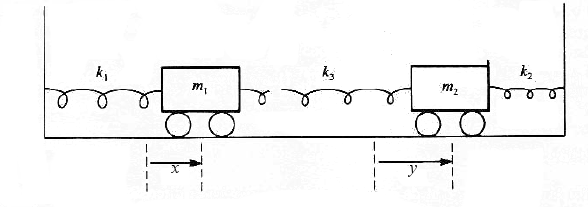
\includegraphics[scale=.4]{imagenes/osci_aco.png}
\end{center}
\end{frame}

\begin{frame}{Osciladores armónicos acoplados}
Se nos presentó un sistema de ecuaciones de segundo orden. Vamos a poder convertirlo en una ecuación pagando el precio de incrementar el orden. El procedimiento es derivar \eqref{eq:sis1} (obviamente es lo mismo empezar por \eqref{eq:sis2}) dos veces respecto a $t$. En el resultado sustituímos $y''$ por su igual según \eqref{eq:sis2}. El resultado es una ecuación que todavía tiene la variable $y$, pero podemos usar \eqref{eq:sis1} para sustituir $y$ por una expresión que sólo tiene $x$ y sus derivadas. Todo esto lo haremos con SAGE.
\end{frame}


\begin{frame}[fragile]{Osciladores armónicos acoplados}
\begin{sageblock}
  x,y,t,m1,m2,k1,k2,k3=\
  var('x,y,t,m1,m2,k1,k2,k3')
  x=function('x',t)
  y=function('y',t)
  eq1=m1*x.diff(2)==-k1*x+k3*(y-x)
  eq2=m2*y.diff(2)==-k2*y-k3*(y-x)
  sust1,=solve(eq2,y.diff(2))
  sust2,=solve(eq1,y)
  eq3=eq1.diff(t,2).subs_expr(sust1).\
  subs_expr(sust2).simplify_full()
\end{sageblock}
Obtenemos la ecuación de cuarto orden
\[{\scriptstyle \sage{eq3}}\]
\end{frame}


\begin{frame}[fragile]{Osciladores armónicos acoplados}
 Vamos a suponer todos los parámetros igual a 1. Encontremos y resolvamos la ecuación característica
\begin{sageblock}
  eq4=eq3.subs(m1=1,m2=1,k1=1,k2=1,k3=1)
  r=var('r')
  z=e^(r*t)
  eq5=eq4.subs_expr(x==z,x.diff(4)==\
  z.diff(t,4),x.diff(2)==z.diff(t,2))/z
  eq5=eq5.simplify_full()
  sol=solve(eq5,r)
\end{sageblock}
Las soluciones de la ecuación característica son $\sage{sol}$.
\end{frame}



\begin{frame}[fragile]{Osciladores armónicos acoplados}
Según lo que hemos dicho antes, la solución general será
\boxedeq{{\scriptstyle x=\sage{x}}}{eq:sol_gen_arm_aco}
\begin{sageblock}
  A,B,C,D=var('A,B,C,D')
  x=A*cos(t)+B*sin(t)+C*cos(sqrt(3)*t)\
  +D*sin(sqrt(3)*t)
\end{sageblock}
La solución es una superposición de ondas con frecuencias \href{http://es.wikipedia.org/wiki/Conmensurabilidad_(matemática)}{inconmensurables}. Decimos que dos magnitudes no nulas son inconmensurables cuando su cociente es irracional. 



\end{frame}


\begin{frame}{Osciladores armónicos acoplados}
¿Tendra el sistema de osciladores acoplados soluciones periódicas?  Esto nos lleva a una pregunta más general. Si $f,g:\rr\to\rr$ son funciones periódicas de período $T_1$y $T_2$, será $f+g$ períodica. La respuesta es el Teorema de abajo. 
  
\begin{thm}  Si $f,g:\rr\to\rr$ son funciones no constantes, periódicas y continuas de período $T_1$ y $T_2$, la función $f+g$ será períodica si y sólo si $T_1$ y $T_2$ son conmensurables.
\end{thm}

\textbf{Dem.} La demostración descansa sobre varios hechos, que poco tienen que ver con las ecuaciones diferenciales. Pero, el Teorema nos parece tan interesante, que vamos a dar algunos detalles y otros los dejaremos como ejercicio.



\end{frame}



\begin{frame}{Osciladores armónicos acoplados}

\textbf{Ejercicio} Sea $F:\rr\to\rr$ una función períodica y sea $\mathfrak{P}$ el conjunto de todos los períodos. Entonces
\begin{enumerate}
 \item $\mathfrak{P}$ es un subgrupo aditivo  de $\rr$. Si $F$ es continua $\mathfrak{P}$ es cerrado. 
 \item Si $\mathfrak{P}$ es cualquier subgrupo aditivo propio y cerrado de $\rr$  entonces  $\mathfrak{P}$ es un grupo ciclico, es decir existe $a>0$ con $\mathfrak{P}=a\mathbb{Z}$.  Como corolario, si $\mathfrak{P}$ es cualquier subgrupo  aditivo cerrado propio  y $T_1,T_2\in \mathfrak{P}$ entonces $T_1$ y $T_2$ son conmensurables. \emph{Ayuda:} Considerar
\[a:=\inf\{x\in \mathfrak{P}:x>0\}\]
Entonces si $a>0$,  $\mathfrak{P}=a\mathbb{Z}$ y si $a=0$,  $\mathfrak{P}=\rr$. 

¿Qué ocurrirá si no suponemos $\mathfrak{P}$ cerrado? 

 \item Demostrar el Teorema. \emph{Ayuda:} Supongamos  que $f+g$ tiene período $T>0$. Entonces:
\[F(x):=f(x+T)-f(x)=g(x)-g(x+T).\]
y por consiguiente $F$ tendrá períodos $T_1$ y $T_2$. 
 \end{enumerate} 
 

\end{frame}


\begin{frame}{Osciladores armónicos acoplados}
Retornando al oscilador armónico y a su solución general \eqref{eq:sol_gen_arm_aco}, el ejercicio anterior nos dice  que la solución no será periódica, a menos que $A=B=0$ o $C=D=0$. 

Estos casos especiales de soluciones se denominan \href{http://es.wikipedia.org/wiki/Modo_normal}{modos normales}.  Usemos SAGE para encontrar y graficar algunos modos normales. 

Gráficaremos las soluciones sobre el espacio de configuraciones. Esto es decir que graficaremos las curvas $t\mapsto (x(t),y(t))$. 



 

\end{frame}

\begin{frame}[fragile]{Osciladores armónicos acoplados}

\textbf{Primer modo normal}

\begin{sageblock}
  x1=x.subs({A:1,B:0,C:0,D:0})
  y1=x1.diff(t,2)+2*x1
  gra=parametric_plot([x1,y1],(t,0,10*pi))
\end{sageblock}

\begin{tabular}{m{3cm} m{6cm}}
\sageplot[scale=.2]{gra} & Los desplazamientos de las dos masas estan sobre la recta $y=x$, vale decir las masas se mueven perfectamente en fase.
 \end{tabular}
 \begin{center}
   \animategraphics[controls, scale=.4]{15}{osciladores_acoplados/primero/modo1-}{0}{9}
 \end{center}

\end{frame}

\begin{frame}[fragile]{Osciladores armónicos acoplados}

\textbf{Segundo modo normal}

\begin{sageblock}
  x1=x.subs({A:0,B:0,C:1,D:0})
  y1=x1.diff(t,2)+2*x1
  gra=parametric_plot([x1,y1],(t,0,10*pi))
\end{sageblock}

\begin{tabular}{m{3cm} m{6cm}}
\sageplot[scale=.2]{gra} & Los desplazamientos de las dos masas estan sobre la recta $y=-x$, vale decir las masas se mueven perfectamente fuera de fase. Cuando una alcanza el desplazamiento negativo menor la otra alcanza el mayor positivo.
 \end{tabular}

 \begin{center}
   \animategraphics[controls, scale=.4]{15}{osciladores_acoplados/segundo/modo2-}{0}{9}
 \end{center}


\end{frame}

\begin{frame}[fragile]{Osciladores armónicos acoplados}

\textbf{Fuera de un modo normal}

\begin{sageblock}
  x1=x.subs({A:1,B:0,C:1,D:0})
  y1=x1.diff(t,2)+2*x1
  gra=parametric_plot([x1,y1],(t,0,30*pi))
\end{sageblock}
\begin{tabular}{m{5cm} m{4cm}}
\sageplot[scale=.3]{gra} & Se obtienen gráficas  bonitas llamadas \href{http://es.wikipedia.org/wiki/Curva_de_Lissajous}{Curvas de Lissajous}, que fuera de los modos normales llenan densamente un cuadrado del plano.
 \end{tabular}
\end{frame}


\begin{frame}{Métodos Operacionales}
\begin{tabular}{m{2cm} m{6cm}}
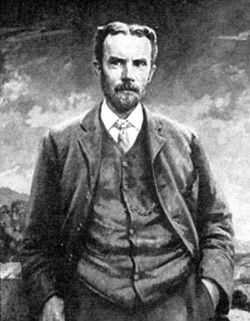
\includegraphics[scale=.6]{imagenes/Heaviside.jpg} &
En las páginas \ref{pag:oper1},  \ref{pag:oper2} y \ref{pag:oper3} hemos empezado a desarrollar una técnica denominada \href{http://en.wikipedia.org/wiki/Operational_calculus}{Método Operacional}. Esta técnica fue iniciada por \href{http://es.wikipedia.org/wiki/Oliver_Heaviside}{Oliver Heavside} (1850-1925).\\
\end{tabular}

Hemos mencionado que una ecuación lineal de orden $n$ con coeficientes constantes y  no homogénea se puede pensar como
\boxedeq{p(D)y=r(x),}{eq:lin_oper}
 donde $p(D)=D^n+p_{n-1}D^{n-1}+\cdots+p_1D+ p_0$ es un operador diferencial polinomial.



\end{frame}

\begin{frame}{Métodos Operacionales}
La idea central del método es proceder desde una manera puramente formal, para afirmar que si $y$ resuelve
\eqref{eq:lin_oper} entonces 
\boxedeq{y=\frac{1}{p(D)}r(x),}{eq:oper_inv}
Esto no parece más que un juego de símbolos del que no se puede desprender nada interesante. Vamos a ver que no es ese el caso. 

El símbolo $1/p(D)$ debería ser interpretado como el operador inverso de $p(D)$. Por ejemplo, supongamos que $p(D)=D$. entonces $p(D)y=y'$. En este caso $1/p(D)$ puede ser definido como

\boxedeq{\frac{1}{p(D)}r=\int r(x)dx}{eq:oper_inv_int}




\end{frame}


\begin{frame}{Métodos Operacionales}
Si tuviesemos $p(D)=D-q$, $q\in\rr$, entonces $p(D)y=y'-qy$. En este caso, teniendo en mente que $y(x)=(1/p(D))r(x)$ debería resolver la ecuación lineal de primer orden $y'-qy=r(x)$, y por la fórmula explícita que obtuvimos para esta solución, es natural definir
\boxedeq{\frac{1}{p(D)}r=e^{qx}\int e^{-qx}r(x)dx}{eq:oper_inv_lin}

Supongamos ahora que $p$ es un polinomio que se factoriza en monomios de primer orden
\[p(D)=(D-p_0)\cdots(D-p_k).\]
Estamos en condiciones de definir 
\boxedeq{\frac{1}{p(D)}r=\frac{1}{D-p_0}\left(\frac{1}{D-p_1}\left(\cdots\frac{1}{D-p_k}\left(r  \right)\cdots    \right)  \right)}{eq:oper_inv_fact}
\end{frame}


\begin{frame}[fragile]{Métodos Operacionales, ejemplo}
 \textbf{Problema.} Resolver  $y''-3y'+2y=xe^x$. Por supuesto que las cuentas las haremos con SAGE. Primero veamos si el polinomio se factoriza



\begin{sageblock}
P.<D>=PolynomialRing(QQ,"D")
p=D^2-3*D+2
q=p.factor()
\end{sageblock}

Vemos que $p=\sage{q}$. Ahora programemos la fórmula \eqref{eq:oper_inv_lin} y usemosla para resolver la ecuación.
\begin{sageblock}
  x=var('x')
  LinInv=lambda r,a: e^(a*x)* (e^(-a*x)*r )\
  .integral(x)
  y=LinInv(LinInv(x*e^x,1),2)
\end{sageblock}

Deducimos $y=\sage{y}$ es solución. 

\end{frame}


\begin{frame}[fragile]{Métodos Operacionales, ejemplo}
 Veamos si es verdad
\begin{sagecommandline}
  sage: (y.diff(x,2)-3*y.diff(x)+2*y).simplify_full()
  x*e^x
\end{sagecommandline}


\end{frame}

\begin{frame}[fragile]{Métodos Operacionales, fracciones simples}
 Otra idea es descomponer $1/p(D)$ en fracciones simples.
\[\frac{1}{(D-p_0)\cdots(D-p_k)}=\left\{\frac{1}{(D-p_0)}+\cdots+\frac{1}{(D-p_k)}\right\}.\]
Como cada témino del miembro de la derecha lo tenemos definido, sólo tenemos que sumar cada uno de ellos. Reprocesemos con esta idea el  ejemplo de antes.
\begin{sageblock}
  q=(1/p).partial_fraction_decomposition()
\end{sageblock}
 Esto nos da la descomposición en fracciones simples
\[\sage{q}.\]
El output es una lista con dos componentes. Recordar que cuando uno descompone una función racional $P(X)/Q(X)$ en fracciones simples resulta en una expresión de la forma $P_0(X)+R(x)$, donde $P_0$ es un polinomio y $R(X)$ es hablando mal y pronto la parte propiamente fraccionaria. 
\end{frame}

\begin{frame}[fragile]{Métodos Operacionales, fracciones simples}
En nuestro caso
\[\frac{1}{p(D)}=\sage{q[1][0]}+\sage{q[1][1]}.\]  
Entonces la siguiente expresión debería darnos una solución 
\begin{sageblock}
  z=LinInv(x*e^x,2)-LinInv(x*e^x,1)
\end{sageblock}
Chequeemos si esto es asi 
\begin{sagecommandline}
  sage: (z.diff(x,2)-3*z.diff(x)+2*z).simplify_full()
  x*e^x
\end{sagecommandline}
¿Será la misma solución que obtuvimos antes?
\begin{sagecommandline}
  sage: bool(y==z)
  True
\end{sagecommandline}
\end{frame}
\begin{frame}[fragile]{Métodos Operacionales, series}
En algunas ocasiones es conveniente desarrollar en serie $1/p(D)$:
\boxedeq{\frac{1}{p(D)}r(x)=\left(a_0+a_1D+a_2D^2+\cdots \right)r(x).}{eq:des_serie}
Por ejemplo es conveniente cuando $r$ es un polinomio, puesto que salvo una cantidad finita, todas las derivadas de $r$ son cero.

\textbf{Ejemplo.} Resolver $y'''+2y''+y=x^4+2*x+5$. 
Como $r$ es un polinomio de grado 4, desarrollemos en serie $1/p(D)$ hasta ese orden

\begin{sageblock}
D=var('D')
L=(1/(1+2*D^2+D^3)).\
taylor(D,0,4).coefficients()
\end{sageblock}
Obtenemos los siguientes coeficientes asociados a cada exponente $\sage{L}$.


\end{frame}


\begin{frame}[fragile]{Métodos Operacionales, series}

Ahora el siguiente código evalúa el segundo miembro de  \eqref{eq:des_serie}
\begin{sageblock}
r=x^4+2*x+5
y=sum([k[0]*r.diff(x,ZZ(k[1])) for k in L])
#ZZ convierte a entero 
    
\end{sageblock}
Llegamos a la solución
\[y=\sage{y}\]
Veamos si es correcta
\begin{sagecommandline}
  sage: bool(y.diff(x,3)+2*y.diff(2)+y==r)
  True
\end{sagecommandline}

\end{frame}
\end{document}

